\documentclass[10pt,twocolumn,a4paper]{article}
\usepackage[utf8]{inputenc}
\usepackage[T1]{fontenc}
\usepackage[provide=*,spanish]{babel}
\usepackage{lmodern,microtype,amsmath,amssymb,graphicx,booktabs}
\usepackage[margin=1.8cm,columnsep=.65cm]{geometry}
\usepackage{authblk,fancyhdr,caption}
\usepackage[colorlinks=true,urlcolor=blue,citecolor=blue,linkcolor=blue]{hyperref}
\setlength{\parindent}{1em}
\setlength{\parskip}{0pt}\raggedbottom
\setlength{\emergencystretch}{1em}
\captionsetup{font=small,labelfont=bf}
\pagestyle{fancy}\fancyhf{}
\fancyhead[L]{\small Evaporación y exceso bariónico}
\fancyhead[R]{\small A. G. García}
\fancyfoot[L]{\footnotesize Estudio exploratorio reproducible | 13 de octubre de 2026}
\fancyfoot[R]{\thepage}
\setlength{\headheight}{14pt}
\newcommand{\nb}{{n_{\bar B}}}
\newcommand{\Y}{{Y_\Delta}}
\newcommand{\sbar}{\bar s}
\title{\Large\bfseries Evaporación simétrica y dilución entrópica del exceso bariónico entre 50 y 30 MeV}
\author{Andrés Germán García}
\affil{\small Investigador independiente, México}
\date{\small 13 de octubre de 2026}
\hypersetup{pdftitle={Evaporación simétrica y dilución entrópica del exceso bariónico},pdfauthor={Andrés Germán García}}
\renewcommand{\normalsize}{\fontsize{9.5}{11.2}\selectfont}
\begin{document}
\setlength{\abovedisplayskip}{6pt}
\setlength{\belowdisplayskip}{6pt}
\twocolumn[
\begin{center}
{\Large\bfseries Evaporación simétrica y dilución entrópica del exceso bariónico entre 50 y 30 MeV\par}
\vspace{8pt}
{Andrés Germán García\par}
\vspace{3pt}
{\small Investigador independiente, México | 13 de octubre de 2026\par}
\end{center}
\begin{abstract}
Se cuantifica el efecto de una inyección térmica sin fuente neta de número bariónico sobre un plasma homogéneo en expansión. Se parte de un baño ideal reducido y se verifica con inventarios HRG completos; se acoplan una población hipotética de agujeros negros no rotantes y una ecuación cinética de producción y aniquilación barión-antibarión. La temperatura inicial es 50 MeV y la integración termina a 30 MeV. En el baño reducido, para una masa inicial de $10^8$ g por agujero negro y cocientes iniciales de energía $f=0$, 0.01, 0.1 y 1, la entropía comóvil del plasma aumenta por factores 1.0000, 1.0109, 1.1093 y 2.0798. El exceso neto por unidad de entropía disminuye en proporción inversa; para $f=1$ pasa de $8.703\times10^{-11}$ a $4.184\times10^{-11}$. Con exceso inicial común, el cruce $n_{\bar B}/(n_B-n_{\bar B})=1$ se desplaza de aproximadamente 38.205 a 37.974 MeV. En una segunda comparación se ajusta el exceso inicial para alcanzar un mismo valor final: el cruce pasa de 38.204 a 39.263 MeV. Su desplazamiento depende, por tanto, de la condición de comparación. La conservación del exceso comóvil es una condición del modelo y la dilución se deduce de sus balances; la integración cuantifica su magnitud. Con el inventario PDG2025, el cruce a exceso final común cambia a 39.269 MeV. Un barrido local de masas identifica un caso con tres cruces debidos al recalentamiento. La neutralidad se verifica por separado en equilibrio con números leptónicos nulos; no se incorpora una red cinética neutral completa. No determina el origen del exceso ni la existencia de ciclos cosmológicos. Se conserva un paquete de código, datos y verificaciones; las incertidumbres físicas del modelo no quedan determinadas por la convergencia numérica.
\end{abstract}
\vspace{.5em}
\noindent\small\textbf{Palabras clave:} exceso bariónico; entropía; evaporación de agujeros negros; cinética de pares; expansión cosmológica.\normalsize
\vspace{1em}]

\section{Introducción}
La diferencia entre las poblaciones de bariones y antibariones no determina por sí sola cuántos pares coexistieron en una época anterior. Para reconstruir esas poblaciones se necesitan relaciones adicionales: temperatura, composición, equilibrio o cinética y condiciones iniciales. Satarov, Mishustin y Greiner \cite{satarov} desarrollan ecuaciones de producción y aniquilación en sistemas en expansión. Yang y Rafelski \cite{yang} sitúan en 38.2 MeV el criterio de igualdad entre antibariones y exceso neto, bajo sus condiciones térmicas y cosmológicas.

Una auditoría previa del autor \cite{garcia} calculó estados de equilibrio con inventarios HRG y un exceso por entropía fijado a partir de una entrada cosmológica. Aquí se emplean cinco pares de densidades redondeadas de esa auditoría como entradas de una extensión cinética reducida. La comparación inicial usa esas entradas reducidas; la sección de robustez reproduce la auditoría y sustituye el cierre tabulado por sumas de los inventarios completos.

La pregunta es cuánto cambian la entropía del plasma, el exceso normalizado y el cruce de abundancias cuando se añade energía por evaporación. La evaporación como fuente de recalentamiento tiene antecedentes explícitos \cite{haque}; este trabajo no introduce ese mecanismo. Su alcance es una comparación numérica controlada con condiciones iniciales comunes, no un ajuste de una historia cosmológica a observaciones.

\section{Modelo de referencia y métodos}
\subsection{Variables y condiciones iniciales}
Se adopta una geometría FLRW plana en expansión, con $a_i=1$ y $T_i=50$ MeV. El tiempo $t=0$ indica el inicio del cálculo, no el Big Bang. Se definen
\begin{align}
\Delta&=n_B-\nb, & \sbar&=s_{\rm pl}/k_B,\\
\Y&=\Delta/\sbar, & S_{\rm pl}&=a^3\sbar,\\
R&=\nb/\Delta, & A&=\frac{\Delta}{n_B+\nb}=\frac{1}{1+2R}.
\end{align}
$S_{\rm pl}$ es la entropía del plasma por volumen comóvil de referencia; no incluye entropía de horizontes ni representa la entropía generalizada total. $A$ mide la asimetría relativa de las poblaciones, mientras que $\Y$ mide el exceso por entropía.

Se fija $\Delta_i=8.8765\times10^{27}$ cm$^{-3}$ y se comparan $f=\rho_{{\rm BH},i}/\rho_{{\rm pl},i}=0$, 0.01, 0.1 y 1. Estas abundancias de agujeros negros son supuestos, no mediciones ni fracciones a su formación. En la primera comparación se usa el mismo exceso inicial; en la segunda se ajusta para alcanzar un exceso por entropía final común.

\subsection{Baño térmico y cierre de equilibrio}
El baño contiene fotones, electrones y positrones sin masa, tres sabores de neutrinos y antineutrinos sin masa, muones masivos y piones neutros y cargados. Sus potenciales químicos se fijan a cero. El sector sin masa tiene $g_*=10.75$. Para cada especie masiva,
\begin{align}
p_j&=\frac{g_jm_j^2T^2}{2\pi^2(\hbar c)^3}
\sum_{k=1}^{64}\frac{c_{j,k}}{k^2}K_2(kx_j),\\
\rho_j&=\frac{g_jm_j^2T^2}{2\pi^2(\hbar c)^3}
\sum_{k=1}^{64}c_{j,k}\left[\frac{3K_2(kx_j)}{k^2}+\frac{x_jK_1(kx_j)}{k}\right],
\end{align}
con $x_j=m_j/T$, $c_{j,k}=1$ para bosones y $(-1)^{k+1}$ para fermiones. Se añaden $\rho_{\rm rel}=\pi^2g_*T^4/[30(\hbar c)^3]$ y $p_{\rm rel}=\rho_{\rm rel}/3$. Se utiliza $\hbar c=1.973269804\times10^{-11}$ MeV cm y $\sbar=(\rho_{\rm pl}+p_{\rm pl})/T$.

Las funciones termodinámicas se tabulan en 1800 temperaturas entre 10 y 100 MeV y se interpolan mediante splines cúbicos. El resultado inicial es $\sbar_i=1.01998166\times10^{38}$ cm$^{-3}$ y $\Y_i=8.70260743\times10^{-11}$. El baño reducido difiere en $-0.1083\%$ del valor de entropía reconstruido de la auditoría; por ello su normalización no coincide exactamente con la del HRG previo.

El producto de equilibrio $b_0(T)^2=n_B^{\rm eq}n_{\bar B}^{\rm eq}$ se reconstruye interpolando $\log\sqrt{n_Bn_{\bar B}}$ mediante PCHIP sobre la tabla \ref{tab:input}. Se adopta un cierre de Boltzmann con $|B|=1$. Fuera de 37--50 MeV se empalma a $T K_2(938.92/T)$ para $b_0$. Los cruces reportados se encuentran dentro del intervalo tabulado; las poblaciones finales a 30 MeV dependen de la extrapolación.

\begin{table}[t]
\centering\small
\caption{Entradas redondeadas de la auditoría térmica \cite{garcia}. Densidades en cm$^{-3}$. No son observaciones.}\label{tab:input}
\begin{tabular}{rrr}\toprule
$T$ (MeV)&$n_B$&$n_{\bar B}$\\\midrule
37&$4.4167\times10^{27}$&$1.1116\times10^{27}$\\
38.203739&$7.3454\times10^{27}$&$3.6727\times10^{27}$\\
40&$1.9166\times10^{28}$&$1.4894\times10^{28}$\\
45&$2.8323\times10^{29}$&$2.7694\times10^{29}$\\
50&$2.7261\times10^{30}$&$2.7172\times10^{30}$\\\bottomrule
\end{tabular}
\end{table}

\subsection{Evaporación y expansión}
Cada agujero negro comienza con masa $M_i=10^8$ g. Se usa la aproximación semiclasica \cite{cai}
\begin{align}
\dot M&=-\alpha/M^2,\\
\alpha&=(5.34\times10^{25})(15.35)\;\mathrm{g^3\,s^{-1}},\\
\tau&=\frac{M_i^3}{3\alpha}=4.066578\times10^{-4}\;\mathrm{s}.
\end{align}
$\tau$ es la vida restante desde $M_i$, no una edad cosmológica inferida. El coeficiente se mantiene constante; no hay acreción, rotación, remanente ni formación posterior de agujeros negros. La aproximación no describe el extremo cuántico de la evaporación.

Con $m=M/M_i$,
\begin{align}
\rho_{\rm BH}&=f\rho_{{\rm pl},i}m/a^3,\\
Q&=-f\rho_{{\rm pl},i}\dot m/a^3,\\
H^2&=\frac{8\pi G}{3c^2}(\rho_{\rm pl}+\rho_{\rm BH}),\qquad H>0,\\
\dot\rho_{\rm pl}+3H(\rho_{\rm pl}+p_{\rm pl})&=Q.
\end{align}
En Friedmann, las densidades de energía se convierten de MeV cm$^{-3}$ a erg cm$^{-3}$. Toda la energía perdida se deposita instantáneamente en el baño: $f_{\rm dep}=1$. Esto idealiza la termalización y omite pérdidas en canales desacoplados. La ecuación complementaria es $\dot\rho_{\rm BH}+3H\rho_{\rm BH}=-Q$; al sumar, se recupera el balance energético del sistema reducido.

\subsection{Cinética barión-antibarión}
Se integra
\begin{equation}
\dot\nb+3H\nb=\langle\sigma v\rangle\left[b_0^2-\nb(\nb+\Delta)\right],
\end{equation}
con la parametrización de Satarov et al. \cite{satarov}, ec. (9),
\begin{equation}
\langle\sigma v\rangle=\left(3.5+8.6\sqrt{T/(939\;\mathrm{MeV})}\right)\mathrm{fm^2}\,c.
\end{equation}
El código convierte fm$^2$ a cm$^2$ y usa $c$ en cm s$^{-1}$. La tasa nucleónica se aplica de forma efectiva a toda la población bariónica. El término inverso permite producción térmica de pares. No se incluye una fuente directa de bariones y antibariones de cascadas de Hawking ni una fuente neta de número bariónico.

Se impone exactamente
\begin{equation}\label{eq:net}
\Delta=\Delta_i/a^3,\qquad n_B=\nb+\Delta.
\end{equation}
La condición inicial corresponde a equilibrio químico compatible con el producto tabulado y ese exceso:
\begin{equation}
\nb_i=\frac{2b_0(T_i)^2}{\sqrt{\Delta_i^2+4b_0(T_i)^2}+\Delta_i}.
\end{equation}
Esta expresión evita cancelación numérica. Los pares son un sector de prueba: se omite su retroacción sobre la energía y la entropía del baño.

\subsection{Identidad entrópica y método numérico}
Los balances anteriores y el baño con potenciales químicos nulos implican
\begin{align}
\frac{dS_{\rm pl}}{dt}&=\frac{a^3Q}{T},\\
\frac{\Y(t)}{\Y_i}&=\frac{S_{{\rm pl},i}}{S_{\rm pl}(t)},\label{eq:dil}
\end{align}
\begin{equation}
\dot\Y=-\Y\frac{Q}{T\sbar}.
\end{equation}
Por tanto, con $Q\geq0$ y exceso positivo, $\Y$ no aumenta. Este resultado es analítico dentro del modelo, no una inferencia estadística ni una nueva ley física.

Se usa \texttt{solve\_ivp} de SciPy con BDF. Durante la evaporación se integra en $u=1-M/M_i$, con $dt/du=3\tau(1-u)^2$, para regularizar la potencia divergente al final. Se evoluciona $N=\ln a$, $T$, $z=a^3\nb/10^{30}$ y una estimación independiente de $S_{\rm pl}/S_{{\rm pl},i}$. Tras la evaporación se integra en $N$ hasta $T=30$ MeV.

La tolerancia relativa es $2\times10^{-7}$; las absolutas son $10^{-10}$, $10^{-8}$, $10^{-14}$ y $10^{-10}$ para las cuatro variables durante la evaporación. Se repite $f=1$ con tolerancia relativa diez veces menor. El paso máximo es 0.008 en cada variable independiente. Se exportan 1201 muestras por caso. En esta revisión el cruce se localiza con Brent sobre la salida densa del integrador, resolviendo $z=\Delta_i/10^{30}$; no se interpola únicamente sobre las muestras exportadas.

\subsection{Comparación con exceso final común}
Se adopta como condición final $\Y_{\rm obj}=(6.12\times10^{-10})/7.04=8.693181818\times10^{-11}$, conservando la entrada de la auditoría previa \cite{garcia}. Su aplicación a 30 MeV supone conservación posterior del exceso comóvil y de la entropía considerada; no es una medición directa a esa temperatura.

Como los pares no retroactúan sobre el baño, el factor $F(f)=S_{{\rm pl},f}/S_{{\rm pl},i}$ es independiente de $\Delta_i$ dentro de este modelo. Se usa el factor de la primera corrida para fijar
\begin{equation}\label{eq:boundary}
\Delta_i(f)=\sbar_i F(f)\Y_{\rm obj}.
\end{equation}
Se reintegran las cuatro condiciones, recalculando las poblaciones iniciales de equilibrio, toda la cinética y los cruces. La abundancia final común es una condición de contorno impuesta, no una predicción independiente. La coincidencia numérica final verifica su implementación. Se repite también el caso $f=1$ con tolerancia menor y el mismo $\Delta_i$, sin reajustarlo.

\section{Resultados}
\subsection{Entropía y exceso normalizado}
La tabla \ref{tab:results} resume las soluciones y la figura \ref{fig:results} muestra sus trayectorias. Sin agujeros negros, la entropía comóvil permanece constante dentro del error numérico. Para $f=0.01$, 0.1 y 1 aumenta aproximadamente 1.09\%, 10.93\% y 107.98\%, respectivamente.

En el caso $f=1$, $S_{{\rm pl},f}/S_{{\rm pl},i}=2.079842$ y $\Y_f=4.184264\times10^{-11}$: una reducción del 51.92\% respecto de $\Y_i$. Esta reducción no representa destrucción del número bariónico neto comóvil. Se conserva $a^3\Delta=\Delta_i$ por construcción y aumenta el denominador entrópico.

\begin{table}[t]
\centering\small
\caption{Resultados a 30 MeV y temperatura del cruce durante la evolución. Decimales para comparación numérica, sin incertidumbre física total asignada.}\label{tab:results}
\begin{tabular}{rrrr}\toprule
$f$&$S_{{\rm pl},f}/S_{{\rm pl},i}$&$\Y_f$&$T_\times$ (MeV)\\\midrule
0&1.0000&$8.703\times10^{-11}$&38.205\\
0.01&1.0109&$8.608\times10^{-11}$&38.202\\
0.1&1.1093&$7.845\times10^{-11}$&38.176\\
1&2.0798&$4.184\times10^{-11}$&37.974\\\bottomrule
\end{tabular}
\end{table}

\begin{figure*}[t]
\centering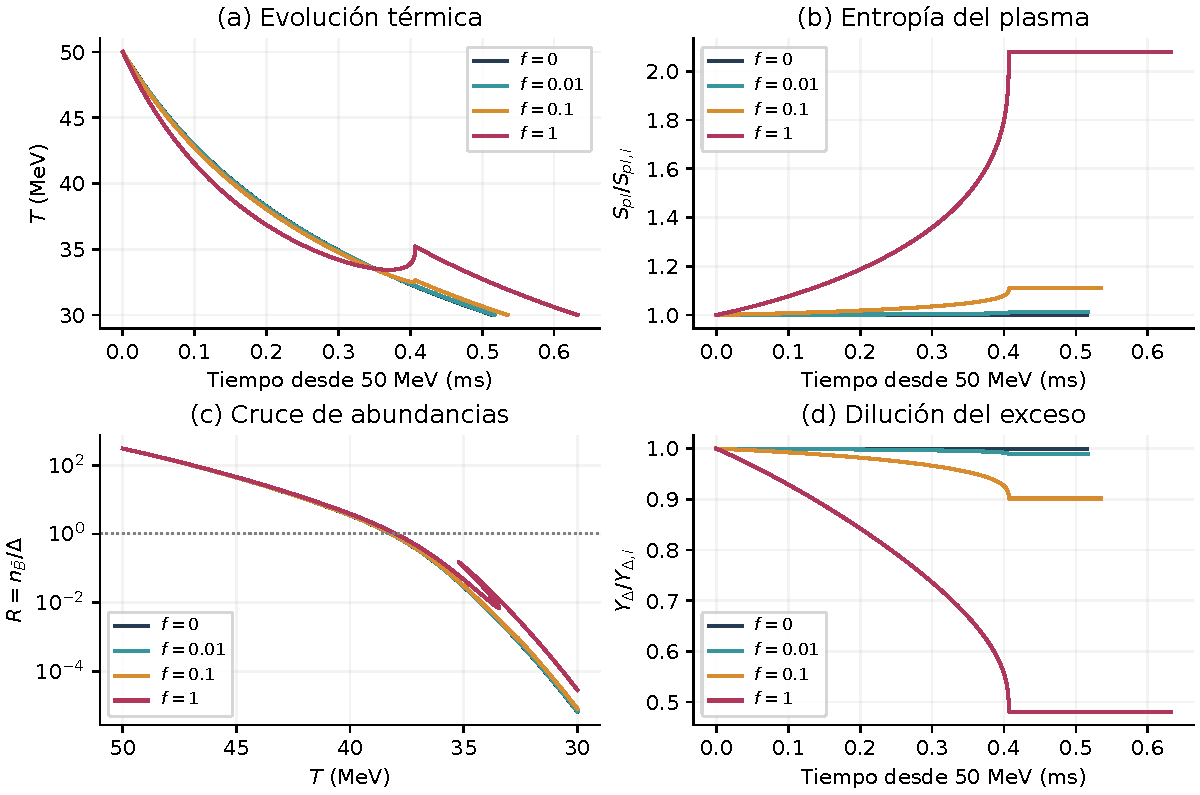
\includegraphics[width=.98\textwidth]{figura_resultados.pdf}
\caption{Trayectorias calculadas con condiciones bariónicas iniciales comunes. (a) Temperatura del plasma, con recalentamiento tardío para $f>0$. (b) Entropía comóvil del plasma. (c) Cociente antibariones/exceso neto; la línea punteada marca $R=1$. (d) Exceso normalizado respecto de su valor inicial. La reciprocidad entre (b) y (d) resulta del balance impuesto. Los distintos casos terminan a 30 MeV en tiempos diferentes; no se representa evolución posterior ni entropía de horizontes.}\label{fig:results}
\end{figure*}

\subsection{Cruce de abundancias y recalentamiento}
El cruce se desplaza aproximadamente $-0.232$ MeV entre $f=0$ y $f=1$. En $R=1$ se cumple $n_B=2\nb$ y $A=1/3$; aún existen antibariones. El cruce no equivale a su desaparición completa ni, por definición, al desacoplamiento químico.

El control arroja 38.2054 MeV y mantiene la proximidad a la referencia 38.2 MeV de Yang y Rafelski \cite{yang}. No constituye una validación independiente: las entradas ya proceden de una reconstrucción térmica cercana a esa referencia, y el baño y los balances químicos difieren entre modelos.

Para $f=1$, el plasma alcanza un mínimo muestreado cercano a 33.44 MeV y luego sube a 35.219 MeV al completarse la evaporación. Después vuelve a enfriarse hasta 30 MeV. Existe recalentamiento parcial; la temperatura nunca supera los 50 MeV iniciales en las trayectorias calculadas. El extremo de emisión instantáneamente termalizada condiciona ese comportamiento.

\subsection{Asimetría relativa y comprobaciones}
En todos los casos $A_i\simeq0.001631$. Para $f=1$, a 30 MeV se obtiene $A_f\simeq0.999942$, mientras $\Y$ se ha reducido. Así, la progresiva dominancia relativa de bariones puede coexistir con dilución entrópica del exceso. Tampoco debe confundirse $a^3\Delta$ constante con $\Delta$ constante: la densidad física cae como $a^{-3}$.

Se reprodujeron exactamente, en el mismo entorno de versiones, las 1201 filas de cada CSV original. El balance entrópico calculado por dos rutas difiere menos de $8.2\times10^{-9}$ en términos relativos. Al reducir la tolerancia, $S_{{\rm pl},f}$ y $\Y_f$ cambian $4.2\times10^{-9}$ relativamente. Las densidades exportadas son positivas.

La localización del cruce sobre salida densa modifica los valores originales entre $1.09\times10^{-4}$ y $1.96\times10^{-4}$ MeV; no cambia las trayectorias ni la conclusión. Para $f=1$ la raíz revisada cambia $1.53\times10^{-8}$ MeV al reducir la tolerancia. La diferencia química máxima muestreada respecto del equilibrio instantáneo es aproximadamente 0.68\% para ese caso, cerca del extremo de emisión. Es una característica de esta idealización, no una predicción robusta de transporte no térmico.

\subsection{Resultados con exceso final común}
La tabla \ref{tab:normalized} presenta las cuatro reintegraciones. El exceso inicial por entropía aumenta desde $8.693\times10^{-11}$ en el control hasta $1.808\times10^{-10}$ para $f=1$. En este último caso la densidad neta inicial requerida es $1.844\times10^{28}$ cm$^{-3}$. El factor entrópico se mantiene, dentro del error numérico, igual al de la comparación anterior.

\begin{table}[t]
\centering\small
\caption{Comparación con $\Y_f=8.69318\times10^{-11}$ impuesto. Las columnas centrales dan el exceso inicial requerido. No se ajustan datos independientes.}\label{tab:normalized}
\begin{tabular}{rrrr}\toprule
$f$&$\Y_i\;(10^{-11})$&$\Delta_i\;(10^{27}\,\mathrm{cm}^{-3})$&$T_\times$ (MeV)\\\midrule
0&8.693&8.867&38.204\\
0.01&8.788&8.964&38.219\\
0.1&9.644&9.836&38.349\\
1&18.080&18.442&39.263\\\bottomrule
\end{tabular}
\end{table}

El cruce aumenta aproximadamente $1.059$ MeV entre el control y $f=1$, frente a la disminución de $0.232$ MeV obtenida con exceso inicial fijo. Para $f=1$, la diferencia entre ambos protocolos es $1.289$ MeV. No existe contradicción: se comparan condiciones bariónicas iniciales distintas. Incluso los controles difieren ligeramente porque ahora se usa exactamente la entrada $\eta/7.04$ en el baño reducido.

El error relativo respecto del valor final objetivo es menor de $5\times10^{-9}$ en las cuatro corridas. La repetición de $f=1$ cambia $\Y_f$ en $5.05\times10^{-10}$ relativamente y $T_\times$ en $8.97\times10^{-8}$ MeV. Las comprobaciones de positividad y del producto de equilibrio inicial se satisfacen. Estas cifras describen precisión computacional, sin asignar exactitud cosmológica a los parámetros.

\begin{figure*}[t]
\centering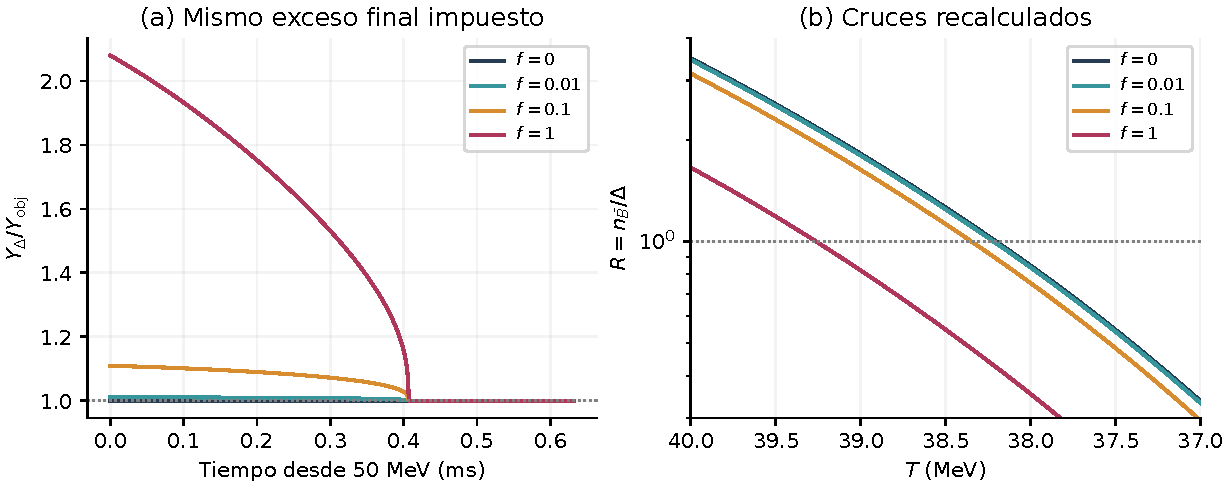
\includegraphics[width=.98\textwidth]{exceso_final_comun/comparacion.pdf}
\caption{Escenarios reintegrados con el mismo exceso por entropía final. (a) Las curvas parten de distintos valores y llegan a $\Y_{\rm obj}$ por construcción. (b) Ampliación del cruce de abundancias: al aumentar $f$, el exceso inicial requerido aumenta y $R=1$ ocurre a mayor temperatura en estos escenarios. Esta comparación mantiene fijos la masa inicial y los demás supuestos del modelo.}\label{fig:normalized}
\end{figure*}

\section{Robustez con inventarios completos}
\subsection{Reproducción e implementación térmica}
Se recuperó el paquete original HRG del autor y se verificaron las huellas SHA-256 de los inventarios PDG2014, PDG2020 y PDG2025 de Thermal-FIST \cite{fist}, fijados en la revisión \texttt{4086191e9522}. Se ejecutó nuevamente la auditoría original, incluidas sus 24 comprobaciones y 1329 registros por especie. Una segunda implementación reproduce las poblaciones y el exceso en cinco temperaturas de los tres catálogos con discrepancia relativa máxima $2.92\times10^{-13}$. Esto es una comparación de implementaciones con datos compartidos, no validación observacional.

El nuevo cálculo incorpora todas las entradas activas de cada inventario, sus antipartículas y el mismo sector leptónico del modelo. Se mantienen masas nominales, anchuras nulas y ausencia de interacciones. No se ejecuta el programa C++ de Thermal-FIST; se usan sus catálogos y una implementación Python.

Para la evolución se tabulan $\rho$, $p$ y $\log b_0$ a potenciales químicos cero en 801 temperaturas entre 20 y 80 MeV, mediante sumas de Bessel de 64 términos. Se usan funciones de Bessel escaladas y se combinan los exponentes de masa y potencial químico antes de evaluar las exponenciales, evitando productos indeterminados en la prueba de 128 términos. Las abundancias proceden directamente de las especies, sin las cinco entradas redondeadas ni extrapolación nucleónica. La integración consulta splines de esa malla densa.

Se mantiene la aproximación de pares como sector de prueba: el baño usa poblaciones de equilibrio a potenciales nulos y no recibe retroacción de la composición cinética. El producto $b_0^2$ conserva el cierre de Boltzmann efectivo. La verificación química descrita abajo cuantifica esa aproximación en estados de equilibrio, sin sustituir una evolución química acoplada.

\subsection{Control de neutralidad en equilibrio}
Se resuelven simultáneamente los potenciales asociados a número bariónico, carga, extrañeza y números leptónicos electrónico y muónico, con
\begin{equation}
\Delta/\sbar=\Y_{\rm obj},\quad n_Q=n_S=n_{L_e}=n_{L_\mu}=0.
\end{equation}
Se toma también $n_{L_\tau}=0$, con neutrinos tau a potencial nulo y sin leptones tau cargados. Para cada especie se usa $\mu_i=B_i\mu_B+Q_i\mu_Q+S_i\mu_S+L_{e,i}\mu_{L_e}+L_{\mu,i}\mu_{L_\mu}$. Los números leptónicos nulos son una elección explícita de control; no se deducen del exceso bariónico. La dependencia de la trayectoria cósmica respecto del estado leptónico está documentada por Wygas et al. \cite{wygas}.

En los estados PDG2025 comprobados entre 30 y 50 MeV, los residuos de carga, extrañeza y números leptónicos son menores de $10^{-7}\Delta$ (los valores obtenidos se sitúan cerca de precisión de máquina). El cruce de equilibrio permanece en 38.203739 MeV: la diferencia respecto del control no neutral es menor de $10^{-8}$ MeV en esta implementación y para los supuestos elegidos. No se extrapola esa insensibilidad a asimetrías leptónicas distintas.

Las correcciones relativas de energía y entropía frente al baño a potenciales nulos son menores de $3.8\times10^{-9}$ y $2.5\times10^{-9}$ en esos puntos de equilibrio. El producto $n_B n_{\bar B}/b_0^2$ difiere de uno menos de $3.5\times10^{-12}$. Son diagnósticos locales de equilibrio; no cotas de error para toda evolución fuera del equilibrio. La neutralidad no se impone dinámicamente en la ecuación efectiva de pares.

\subsection{Reintegración y sensibilidad a la masa}
Para comparar fondos térmicos se fija el mismo $\Y_i=\Y_{\rm obj}$ en el protocolo de exceso inicial común; la densidad inicial se calcula con la entropía de cada fondo. El segundo protocolo mantiene $\Y_f=\Y_{\rm obj}$. En PDG2025, para $M_i=10^8$ g y $f=1$, se obtiene $S_f/S_i=2.079958$, $\Y_i=1.808146\times10^{-10}$ en el protocolo final común, y un cruce de 39.269261 MeV. El cambio frente al fondo reducido es $+0.006241$ MeV. Entre los tres catálogos el rango de ese cruce es aproximadamente 0.000152 MeV; no representa incertidumbre física total.

Se ejecutaron doce combinaciones de masas $M_i=(0.70,0.85,1.00)\times10^8$ g y abundancias $f=0$, 0.01, 0.1 y 1, bajo ambos protocolos: 24 trayectorias. Este barrido local mantiene la evaporación completa antes del punto final de 30 MeV y no representa un intervalo observacionalmente permitido. Se añadieron controles de catálogo, tolerancia y resolución térmica. Las discrepancias numéricas del objetivo final son menores de $2\times10^{-8}$ en el barrido.

\begin{table*}[t]
\centering\small
\caption{Inventario PDG2025, $f=1$ y exceso final común. Se conservan todos los cruces en orden temporal; el tiempo comienza a 50 MeV. Son resultados condicionados al depósito energético instantáneo.}\label{tab:mass}
\begin{tabular}{rrrrl}\toprule
$M_i$ ($10^8$ g)&$S_f/S_i$&$\Y_i$ ($10^{-11}$)&Número de cruces&Temperaturas de los cruces (MeV)\\\midrule
0.70&1.854078&16.11784&1&38.203739\\
0.85&1.955012&16.99528&3&38.846320; 38.541989; 38.203739\\
1.00&2.079958&18.08146&1&39.269261\\\bottomrule
\end{tabular}
\end{table*}

Para $M_i=0.70\times10^8$ g, la evaporación termina a 45.983 MeV, antes del cruce; el exceso por entropía ya alcanzó el objetivo cuando se cruza $R=1$. Para $M_i=0.85\times10^8$ g, $R$ cruza primero hacia abajo, luego hacia arriba durante el recalentamiento y finalmente hacia abajo tras la evaporación (figura \ref{fig:multi}). Los tiempos son aproximadamente 0.187886, 0.237485 y 0.301677 ms. Para $10^8$ g sólo se registra un cruce en el protocolo final común.

Estos resultados obligan a especificar si se informa el primer cruce, el último o todos. Los CSV resumen del barrido identifican el último en las columnas escalares y conservan las listas completas. Un cambio no monótono de abundancias durante una inyección energética no constituye una oscilación cosmológica ni una transición a agujero blanco.

\begin{figure*}[t]
\centering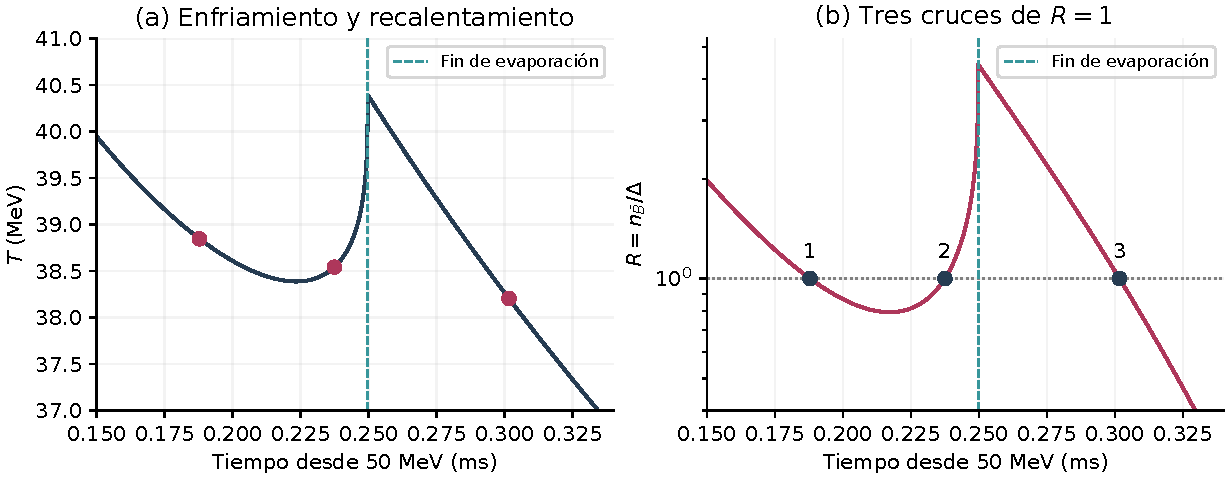
\includegraphics[width=.98\textwidth]{robustez_hrg/resultados/multicruce.pdf}
\caption{Caso $M_i=8.5\times10^7$ g, $f=1$, con exceso final común y fondo HRG PDG2025. (a) Temperatura del plasma. (b) Tres cruces de $R=1$, señalados cronológicamente. La línea vertical indica el fin de evaporación. El comportamiento resulta del enfriamiento, la inyección energética y el reajuste térmico de pares en este modelo.}\label{fig:multi}
\end{figure*}

En el caso de tres cruces, reducir diez veces la tolerancia cambia sus temperaturas menos de $2.3\times10^{-8}$ MeV; duplicar la resolución térmica las cambia menos de $1.6\times10^{-8}$ MeV. La multiplicidad persiste en ambos controles. Para $M_i=10^8$ g y $f=1$, el cambio del cruce al duplicar la malla es menor de $10^{-7}$ MeV. Estos controles descartan una explicación por esas discretizaciones, pero no evalúan transporte no térmico, espectros de Hawking ni termalización finita.

\section{Discusión y alcance}
\subsection{Qué se establece}
El cálculo cuantifica cuánto diluye una inyección energética el exceso normalizado bajo un conjunto explícito de hipótesis. La identidad \eqref{eq:dil} explica el signo del efecto y la integración determina su magnitud mediante la evolución del baño y de la expansión. La contribución es un ejercicio reproducible de consistencia y comparación, sin novedad física fundamental establecida por esta prueba.

La distinción entre $A$ y $\Y$ resuelve una ambigüedad relevante: la eliminación de pares puede hacer más visible el exceso en la composición, pero no crea necesariamente exceso neto nuevo. Si se desea estudiar generación neta, debe introducirse y justificar una fuente en $\dot\Delta+3H\Delta=Q_{\Delta B}$, ausente aquí.

\subsection{Normalización cosmológica}
La auditoría de partida empleó una conexión adiabática entre el exceso temprano y el actual. Esa conexión debe modificarse al añadir entropía. La primera comparación aísla el efecto de $f$ con $\Delta_i$ común; la segunda pregunta qué exceso inicial permite alcanzar el mismo objetivo final. Son dos problemas de contorno diferentes.

La condición \eqref{eq:boundary} ya se implementó mediante nuevas integraciones. Durante estas evoluciones,
\begin{equation}
\Y(t)=\Y_{\rm obj}\frac{S_{{\rm pl},f}}{S_{\rm pl}(t)}.
\end{equation}
Así, antes de completar la inyección se requiere un exceso por entropía superior al final. En los casos calculados, esa normalización modifica el cruce hacia temperaturas mayores, aun cuando la entropía sigue diluyendo $\Y$ a lo largo de cada trayectoria. El sentido del desplazamiento no debe describirse sin especificar qué dato se mantiene fijo.

Ajustar $\Delta_i$ no explica su origen. Diferentes condiciones iniciales y distintas inyecciones entrópicas pueden terminar con el mismo $\Y_f$; ese valor final por sí solo no identifica $f$. Tampoco la coincidencia impuesta valida la existencia de la población de agujeros negros.

\subsection{Límites físicos y cosmológicos}
La evolución cinética conserva una tasa efectiva y no resuelve dinámicamente los balances eléctricos, de extrañeza y leptónicos. Esos balances se resolvieron en controles de equilibrio independientes. La robustez con inventarios completos sustituye el cierre de cinco puntos del modelo de referencia, pero no incorpora interacciones, anchuras de resonancia, transporte ni incertidumbre física total.

La masa y abundancia iniciales de agujeros negros no se vinculan a una historia de formación. La emisión se reduce a un depósito energético homogéneo e instantáneo; no se calculan espectros, cascadas, distribución de masas ni restricciones observacionales de la población. La composición cinética de los pares no retroactúa sobre el baño: el fondo HRG usa su contribución de equilibrio a potenciales nulos. El balance entrópico se refiere al plasma del modelo, no a una evaluación de la segunda ley generalizada.

La rama $H>0$ y los componentes adoptados no incluyen una transición a contracción o rebote. No hay ecuaciones que generen agujeros blancos o universos hijos. Por ello, la ausencia de ciclos en la integración es una consecuencia del alcance, no una refutación general; tampoco el residuo conservado implica ciclos. El intervalo 50--30 MeV no permite inferir el futuro del universo.

\section{Conclusiones}
En las comparaciones realizadas, la evaporación aumenta la entropía comóvil del plasma y diluye el exceso bariónico por entropía. En el baño reducido, para $f=1$, el incremento entrópico es un factor 2.0798 y la dilución del exceso normalizado es 51.92\%; el cruce de abundancias ocurre cerca de 37.974 MeV con exceso inicial común. Al ajustar las condiciones iniciales al mismo exceso final, el caso $f=1$ requiere $\Y_i=1.808\times10^{-10}$ y cruza a 39.263 MeV. Se presenta recalentamiento parcial, sin recuperación de la temperatura inicial.

La reintegración con inventarios completos conserva la dilución y sitúa el cruce del caso de referencia a exceso final común en 39.269 MeV. El barrido de masas muestra que el cruce puede ser múltiple: por ello su temperatura no es una escala universal y debe acompañarse de las condiciones de contorno y la cronología de evaporación.

El número neto comóvil se conserva por hipótesis. La asimetría relativa puede aumentar al disminuir la población de pares mientras el exceso por entropía disminuye. Estas afirmaciones son compatibles y describen cantidades distintas. Los resultados cierran una prueba exploratoria reproducible; no establecen el origen de la asimetría, una nueva ley física ni una cosmología cíclica.

\section*{Datos, código y trazabilidad}
El suplemento contiene \texttt{simular.py}, los cuatro CSV, resultados JSON, entorno, figuras, fuentes de este manuscrito y la entrada original. Se ejecutó en Linux con Python 3.12.14, NumPy 2.3.5, SciPy 1.17.0 y Matplotlib 3.10.8. El código revisado añade localización de raíces sobre salida densa y un parámetro opcional de exceso inicial. El programa \texttt{ajustar\_exceso\_final.py} ejecuta la segunda comparación y exporta sus datos en una carpeta separada. La carpeta \texttt{robustez\_hrg} incorpora los inventarios originales con licencia y hashes, su reproducción, la nueva implementación térmica, los controles de neutralidad y las trayectorias del barrido. Las instrucciones para Windows se incluyen sin afirmar una ejecución en ese sistema.

\section*{Asistencia en la preparación}
Se utilizó asistencia de inteligencia artificial para la revisión del código, la ejecución, la redacción y la composición. La interpretación científica y la decisión de publicación corresponden al autor. Esta revisión incorpora exceso final común, inventarios completos y sensibilidad a masa y abundancia; el archivo de la auditoría previa no se modifica.

\begin{thebibliography}{9}\small
\bibitem{satarov} L. M. Satarov, I. N. Mishustin y W. Greiner (2013). Evolution of antibaryon abundances in the early Universe and in heavy-ion collisions. \textit{Physical Review C} \textbf{88}, 024908. \href{https://doi.org/10.1103/PhysRevC.88.024908}{doi:10.1103/PhysRevC.88.024908}.
\bibitem{yang} C. T. Yang y J. Rafelski (2022). Cosmological strangeness abundance. \textit{Physics Letters B} \textbf{827}, 136944. \href{https://doi.org/10.1016/j.physletb.2022.136944}{doi:10.1016/j.physletb.2022.136944}. Sección 3 y figura 3.
\bibitem{garcia} A. G. García (2026). \textit{Baryon-Antibaryon Reconstruction at 50 MeV: Rest Masses and Cosmological Abundances}. Manuscrito del autor, fechado 9 de octubre de 2026, tabla 2; archivo aportado \texttt{Baryon\_Antibaryon\_Thermal\_Audit\_EN(1).pdf}. Fuente interna de datos, sin revisión externa verificada.
\bibitem{haque} M. R. Haque, E. Kpatcha, D. Maity y Y. Mambrini (2023). Primordial Black Hole Reheating. \href{https://arxiv.org/abs/2305.10518}{arXiv:2305.10518}. Referencia de contexto; su escenario inflacionario no se reproduce.
\bibitem{cai} Y.-F. Cai, C. Chen, Q. Ding y Y. Wang (2022). Ultrahigh-energy gamma rays and gravitational waves from primordial exotic stellar bubbles. \textit{European Physical Journal C}. \href{https://doi.org/10.1140/epjc/s10052-022-10395-w}{doi:10.1140/epjc/s10052-022-10395-w}; \href{https://arxiv.org/abs/2105.11481}{arXiv:2105.11481}, apéndice B, ecs. (B3)--(B4). Sólo se toma la parametrización de pérdida de masa.
\bibitem{fist} V. Vovchenko y H. Stoecker (2019). Thermal-FIST: A package for heavy-ion collisions and hadronic equation of state. \textit{Computer Physics Communications} \textbf{244}, 295--310. \href{https://doi.org/10.1016/j.cpc.2019.06.024}{doi:10.1016/j.cpc.2019.06.024}. Catálogos fijados del paquete del autor, con hashes incluidos.
\bibitem{wygas} M. M. Wygas, I. M. Oldengott, D. B\"odeker y D. J. Schwarz (2018). Cosmic QCD Epoch at Nonvanishing Lepton Asymmetry. \textit{Physical Review Letters} \textbf{121}, 201302. \href{https://doi.org/10.1103/PhysRevLett.121.201302}{doi:10.1103/PhysRevLett.121.201302}. Contexto del papel de los números leptónicos, sin reproducir su análisis de QCD.
\end{thebibliography}
\end{document}
